\chapter{Aktueller Forschungsstand}\label{forschungsstand}
Wie bereits erwähnt gibt es zwei Wissenschaftliche Ansätze um Verschlüsselungsverfahren vor der Rechenleistung von Quantencomputern sicher zu machen, \ac{PQC} und \ac{QKD}. Dieses Forschungsprojekt soll die \ac{QKD} im Rahmen einer fiktiven Implementierung für die Hochschule München erproben.

Wie der Technischen Richtline des Bundesamts für Sicherheit in der Kommunikationstechnik [BSI1] zu entnehmen ist, werden alle Verschlüsselungsverfahren welche auf ein gemeinsames Passwort basieren (so gennante symmetrische Verfahren) mit der Rechenleistung der Quantencomputer leicht innerhalb weniger Sekunden entschlüsselbar.
Grund hierfür ist, dass sich solche Verfahren auf pseudozufällige Zahlen stützen. Zufällige Zahlen können mit konventionellen Computersystemen nicht zuverlässig erzeugt werden. Diese werden mithilfe von mathematischen Algorithmen simuliert, hierdurch entsehen sogennante Pseudozufallszahlen (https://users.fmi.uni-jena.de/~hinze/fv-hinze.pdf)[bibtext machen].
Mit genügend Recheneleistung lassen sich solche Zufallszahlen allerdings satistisch ermitteln um eine Verschlüsselung rückgangig zu machen.(https://www.cs.uni-potsdam.de/ti/lehre/07-Kryptographie/slides/slides-2.3-anim.pdf).

Quantencomputersysteme könnten in naher Zukunft die benötigte Rechenleistung haben um solche Verschlüsselungen mit "Pseudozufallszahlen" innerhalb küzester Zeit zu knacken. Hinzu kommt, dass ein solcher Schlüssel abhörsicher über öffentliche Kanäle (bspw. das Internet) übermittelt werden muss um kein unerwünschtes Entschlüsseln der Nachricht garantieren zu können.[Bsi2]

Bereits seit Mitte der 80er gibt es das erste Übertagungsprotokoll um "echt" zufällig generierte Schlüssel zu erzeugen und ein Abhören des Signals garantiert ausschließen können.
Hiermit ist die Basis für eine mathematisch beziehungsweise statistisch perfekte Verschlüsselung geschaffen.(https://mpl.mpg.de/fileadmin/user_upload/Chekhova_Research_Group/Lecture_4_12.pdf) Das generieren einer "echt" zufälligen Zahl basiert auf dem Prinzip der Messung von Polarisationszuständen, dessen Ergebnis auf Grund der quantenmechanischen Eigenschaften von Photonen nicht bekannt und nicht vorhersagbar ist. Durch eine gemeinsame Polarisation der Signale die von den Schlüsselaustauschenden empgfangen werden, kann erreicht werden, dass sich beide Signale bei gleicher Messung gleich verhalten. Beide Signale haben also den selben Zustand unabhängig davon wie weit sie voneinander entfernt sind, dieses Prinzip nennt man Quantenverschränkung.
https://www.spektrum.de/news/wie-real-ist-die-quantenverschraenkung/1445463

Die Besonderheit liegt hier bei der sehr hohen Wahrscheinlichkeit den Schlüssel durch äußere Abhörversuche unbrauchbar zu machen, hiermit wird das unbemerkte Abhören beim Schlüsselaustausch unmöglich. Im Englischen bezeichnet man besagte Verfahren als \ac{QKD}.

Das Kernverfahren der Quantenkryptographie liegt in dieser Schlüsselgenerierung
welche, analog zu den konventionellen Verschlüsselungsverfahren, dem Austausch einer gemeinsamen Zufallszahl dient mit der eine beliebige Nachricht verschlüsselt werden kann. Die verschlüsselte Nachricht ist ohne den Schlüssel nitcht entschlüsselbar und kann nun über einen öffentlichen Kommunikationsweg (beispielsweise das Internet) übertragen werden, siehe Abbildung \ref{fig:Bild1}. 

\begin{figure}[htbp] 
  \centering
     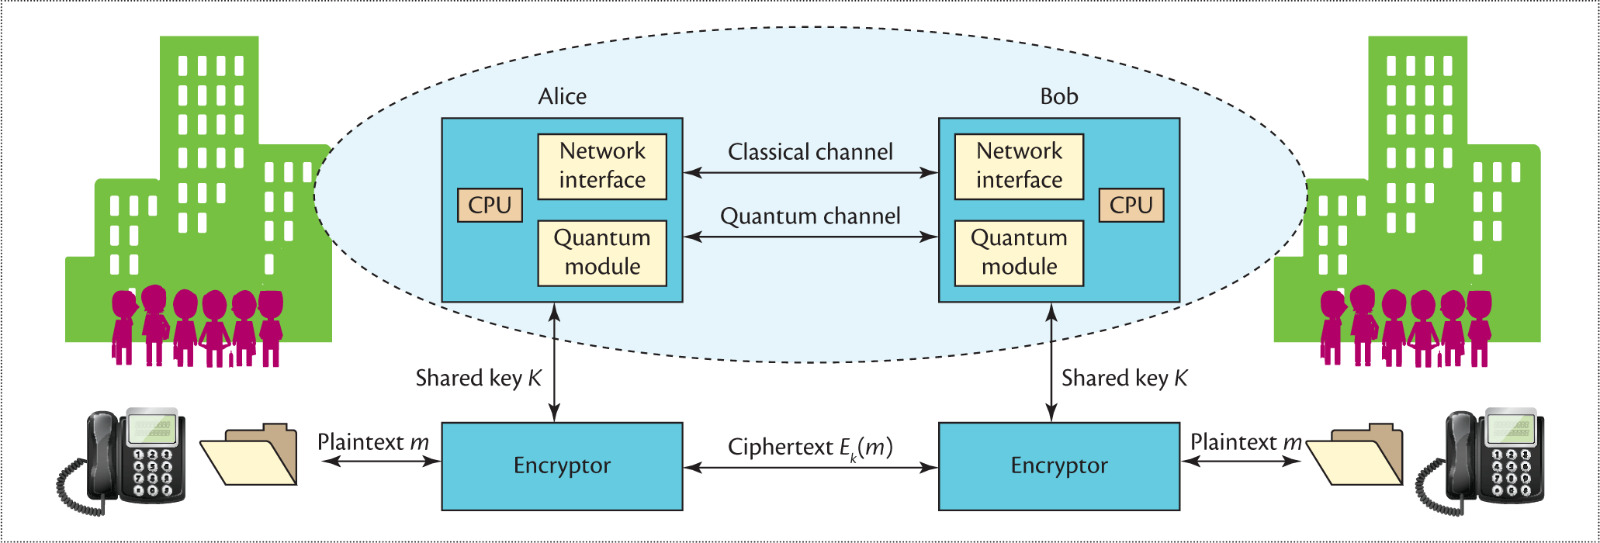
\includegraphics[width=0.9\textwidth]{img/qkd.jpg}
     \caption{Quantum Schlüsselaustausch (QKD) System. Die Architektur setzt sich zusammen aus einem Sender, Alice, und einem Empfänger, Bob, einem Optischen Quanten Kanal und einem Klassischen Kanal.}
  \label{fig:Bild1}
\end{figure}

Das Erzeugen, Übertragen und Messen von solchen verschränktten Photonen bedarf jedoch spezieller Gerätschaften und kann weder über Kupferleitungen noch die konventionellen Gerätschaften welche benutzt werden um Signale über Glasfaserleitungen zu übertragen.
Aktuell werden in der Forschung zwei verschiedene Ansätze verfolgt. Das verschränktte Signal kann entweder über den Luftweg mittels zwei zueinander ausgerichteten Teleskopen oder über Lichtwellenleiter übertragen werden, wenn an beiden Enden die entprechenden Gerätschaften zum messen der Polarisation vohanden sind. Man spricht in diesem Kontext auch von Quantennetzwerken.

Zusammenfassend kann man also festlegen:
\ac{QKD} benötigt neuartige Netzwerkstrukturen zur Übertragung Quantenverschränkter Signale. 
Fas Prinzip der \ac{QKD} verspricht ein außergewöhnliches (mathematisch perfektes) Sicherheitsniveau mithilfe quantenphysikalischer Mechasnismen, welches für herkömmliche Verschlüsselungsmethoden unerreichbar ist.

Die Verschlüsselungalgorithmen werden in den Medien oft als “unknackbar” 
angepriesen. In der Praxis wurde diese Behauptung jedoch für die Implementierungen widerlegt.

In unserem Forschungsprojekt soll erörtert werden wie ein solches Netz funktioniert und beispielhaft für die Hochschule München implementiert werden könnte.
Hieraus ergeben sich mehrere technische Möglichkeiten welche hinsichtlich ihrer Funktionsweise und ihren Sicherheitsmerkmalen erprobt und getestet werden müssen.

Bei der Implementierung eines Quantennetzwerkes sind neben der Sicherheit des Netzes auch weitere Aspekte zu beachten.
So wollen wir neben der Sicherheit auch die Nachhaltigkeit der verschiedenen Übertragungstechniken vergleichen.
Im speziellen sind hier die Aufwände bei der Inbetriebnahme, die benötigte Energie während dem Betrieb und die Zuverlässigkeit bzw. die Qualität des Signals zu nennen.

Die zwei Methoden haben unterschiedliche Vor- und Nachteile, so ist die Übertragung durch einen Lichtwellenleiter bspw. auf wenige 100km beschränkt und die Übertragung durch die Luft benötigt eine Strecke ohne feste, störende Objekte.


\section{Air}

Wie von \cite{Ren_2017} in Kooperation zwischen Wien und Shanghai bewiesen, lassen sich Photonen über Satelliten durch den quasi luftleeren Raum Störungsfreier und dadurch viel weiter übertragen. Im Falle der Studie von \cite{Ren_2017} wurde ein Schlüsselaustausch zwischen Wien und Shanghai über eine Strecke von 1120 Kilometer erreicht werden. Die aktuelle Übertragungsrate ist allerdings mit 0,12 Bit/s sehr gering. Hinzu kommt, dass die Übertragung, aufgrund der Störeffekte der Photonen des Sonnenlichts, nur Nachts möglich ist.

Forscher der Leibniz Universität Hannover haben zusammen mit Forschern der Universität Glasgow und des des japanischen NICT (National Institute of Information and Communications Technology) eine Möglichkeit der Übertragung verschränkter Photonen im Infrarotspektrum geschaffen \cite{prabhakar_two-photon_2020}. Diese Technologie nutzt das so genannte "atmosphärische Fenster" d.h. einen bestimmten Frequenzbereich bei dem sich die Atmosphäre lichtdurchlässiger verhält. Auch die Sonnenstrahlung ist im Infrarotbereich schwächer und stört die Übertragung weniger als im sichtbaren Bereich. Allerdings ist diese Methode noch weniger ausgereift und weißt bei der Detektion eine Rate von 2\% aller Übertragenen Photonen im Gegensatz zu 90\% bei der Methode von \cite{Ren_2017} auf.

Einen

\section{Lichtwellenleiter}

Die Standardmethode für verschlüsselte Kommunikation in Quantennetzwerken ist die \ac{QKD} über Fiberglas.
Hier wird die grundlegende Materie des Lichts, Photonen, übertragen um Informationen weiter zu geben.
Diese Übertragung kann nicht ohne Rauschen stattfinden, sodass ein Übertragung bis maximal 100 km möglich ist\cite{Shen2018}.

Des weiteren findet die Übertragung immer von einem Teilnehmer zu einem zweiten statt und ein Multicast, welcher eine Information von einem Sender an mehrere Empfänger schickt, ist in Quantennetzwerken mit \ac{QKD} nicht etabliert.
Stattdessen werden die Informationen individuell an jeden einzelnen Empfänger gesendet oder Daten werden von einem Verteiler an die verschiedenen Empfänger verteilt.
Dabei muss ein Schlüsselaustausch zwischen dem ersten Teilnehmer und dem Verteiler stattfinden und ein zweiter Schlüsselaustausch zwischen dem Verteiler und dem zweiten Teilnehmer.
Somit ist die Übertragung auf dem Verteiler unverschlüsselt und deshalb muss dem Verteiler vertraut werden\cite{Qiu2018}.

Dieses Jahr wurde ein Netzwerk zwischen acht Teilnehmern realisiert, welches mit multiplexern und demultiplexern arbeitet.
Das hat den Vorteil, dass keine aktives verteilen der einzelnen Daten geschehen muss\cite{Siddarth2020}.

Die Übertragung in einem Lichtwellenleiter kann dabei entweder im single-mode als auch im multi-mode stattfinden.
Beim single-mode wird ein einzelner Photonenstrahl vom Sender in den Lichtwellenleiter gegeben, was ein dünneres Kabel erlaubt.
Allerdings macht die mulit-mode Methode eine höhere Präzession möglich\cite{VanMeter2014}.
Beide Möglichkeiten werden aktuell schon in klassischen Netzwerken genutzt und sind weit verbreitet.

